\documentclass[18pt,oneside,a4paper, titlepage]{article}

\usepackage[hidelinks]{hyperref}
\usepackage[pdftex]{graphicx}

\begin{document}
\begin{figure}[t]
	\centering
	
\includegraphics[scale=0.35]{logo-polimi.png}
\end{figure}
\title{\textbf{TETRIS on STM32F4-Discovery}\\Advanced Operating Systems Project Report\\ A.Y. 2015/2016\\
	Politecnico di Milano}	
\author{Antenucci Sebastiano, matr. 790021\\Cattaneo Michela Gaia, matr. 863116\\Filippo Ciceri, matr. 855162 }
\date{May, 2016}
\maketitle

\newpage
	\tableofcontents

\newpage
\section{Introduction}
	This project aims at implementing the well-known Tetris game on the STM32F429I-Discovery board using Miosix kernel. This board is equipped with:
	\begin{itemize}
		\item high performance ARM Cortex M4 processor with 2D graphics accelerator
		\item 2.4" QVGA TFT LCD display provided with resistive touchscreen
		\item 180Mhz/225 DMIPS execution performance from Flash memory
		\item embedded ST-LINK/V2
	\end{itemize}
	\vspace{1cm}
	\begin{figure}[h]
		\centering
		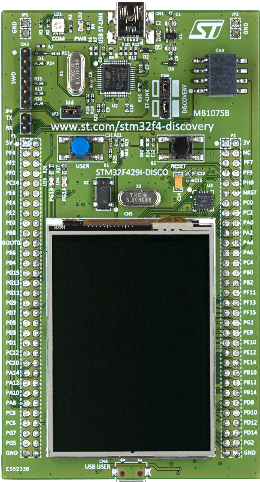
\includegraphics[scale=0.7]{board.jpg}
	\end{figure}
	
\newpage
\section{Tetris game}
	Tetris is a tile-matching puzzle video game.
	\subsection{Gameplay}
		There are seven different pieces of different colors, composed of four square blocks each.\\
		\begin{figure}[h]
			\centering
			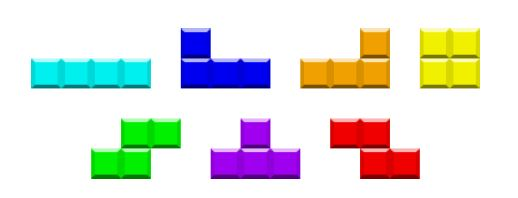
\includegraphics[scale=0.7]{blocks.jpg}
		\end{figure}
		\\
		A random sequence of pieces fall down the playing field and the objective of the game is to translate or rotate the pieces in order to create horizontal lines with no gaps (it is possible to delete more rows simultaneously). When the row is filled, it disappears and any block above gets translated down.\\
		As the game progresses the pieces will not fall faster, as it happens in the classic Tetris game, and there is just one level.\\The game stops when the stack of pieces reaches the top and it is no more possible to add more. 
	\subsection{The game on the board}
		Once the board is connected to power, it displays the starting screen: a touch is expected in order to start a new game.\\
		The LCD display shows the game progress and the touchscreen allows to press the buttons drawn on the bottom of the display in order to translate the current piece or to press the rectangular area in order to rotate the current piece.\\
		The bar at the top of the screen displays the score: 1 point is given when the piece is lied down and 10 points are given when a row is full and canceled.\\
		When it is no more possible to add a new piece on the display, a game over screen will be shown.\\
		In order to start a new game it is necessary to press the reset button.
\newpage
\section{Structure of the program}
	The program is composed of 5 classes, a main (these corresponds to the .cpp files) and 6 .h files.\\
	\vspace{0.5cm}
	\begin{figure}[h]
		\centering
		\includegraphics[scale=0.4]{TetrisClassDiagram.png}
	\end{figure}
	\vspace{0.5cm}
	\\
	The Block class stores the coordinates of the block, its color and its structure. The classic blocks are created by passing the blockID, a number from 0 to 6, which corresponds to a specific block.\\
	The rotate and translate methods
	
	
\newpage
\section{Software and tool used}
	\begin{itemize}
		\item \textbf{miosix-kernel}: OS kernel designed to run on 32bit microcontrollers. (\url{https://miosix.org/})
		\item \textbf{mxgui}: Miosix GUI library.
		\item \textbf{Notepad++}: to write the code.
		\item \textbf{QSTlink2}: to transfer the program to the board. (\url{https://github.com/fpoussin/qstlink2})
	\end{itemize}

\end{document}